\chapter{Pruebas experimentales}
\label{cap:pruebasExpirementales}

En este capítulo se expondrán distintas pruebas realizadas a la herramienta para documentar cómo se comportan los archivos portadores en distintos entornos y analizar su eficacia.\\

A lo largo del capítulo se mencionará el archivo ``pruebas.txt'' siendo el contenido de este:

\begin{verbatim}
PITEA Protección de la informacíon mediante técnicas de esteganografía acústica
Alberto Martin Oruña y Rodrigo Gallego Marin
\end{verbatim}


\section{Transmisión vía radiofrecuencia}
\label{sec:transmision-rf}

En esta sección se hablará de cómo se comportan los archivos portadores al ser transmitidos mediante radiofrecuencia.

\subsection{Generación del archivo portador}

El audio portador ha sido generado como se indica en la figura~\ref{fig:gen_radio}, donde se puede apreciar que se ha generado un archivo de audio en formato WAV tras cifrar la información con el cifrado AES, ocultando el resultado del cifrado mediante el plasmado del texto en una imagen, generando la figura~\ref{fig:text_radio}, y convirtiendo esa imagen en una señal de audio codificada en formato SSTV con 16 bits de profundidad y una frecuencia de 48000 Hz.

\begin{figure}[h]
	\centering
	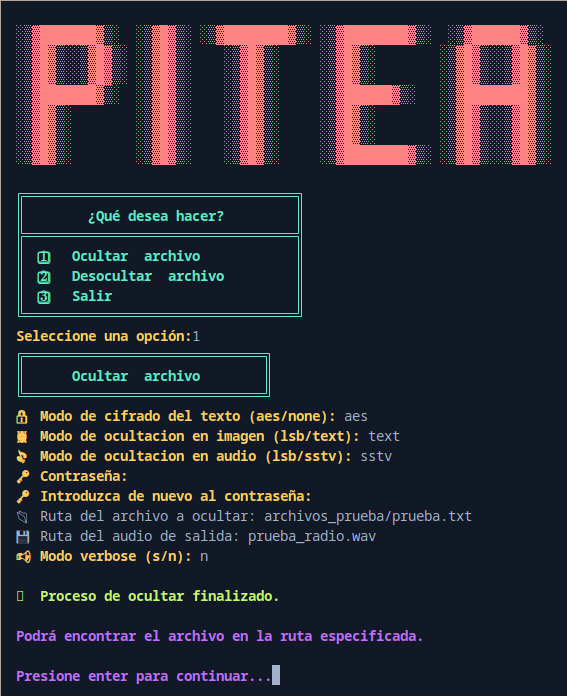
\includegraphics[width = 0.4 \textwidth]{Imagenes/pitea/gen_radio.png}
	\caption[Generación de audio portador, AES, \textit{text}, SSTV.]{Generación de audio portador, AES, \textit{text}, SSTV. Captura de pantalla de la herramienta.}
	\label{fig:gen_radio}
\end{figure}

\begin{figure}[h]
	\centering
	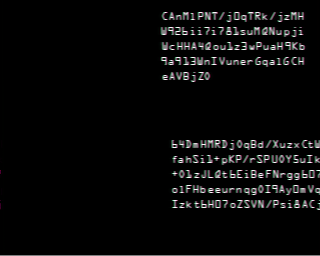
\includegraphics[width = 0.5 \textwidth]{Imagenes/pitea/text_radio.png}
	\caption[Imagen generada por el \textit{OcultadorText}.]{Imagen generada por el \textit{OcultadorText}. Generada por la herramienta.}
	\label{fig:text_radio}
\end{figure}




\FloatBarrier

\subsection{Resultado}


El archivo portador fue transmitido en VHF (\textit{Very High Frecuency}), en la banda de radioaficionados y en la frecuencia destinada a SSTV, con un walkie-talkie\footnote{Baofeng UV-5R (\url{https://baofeng.es/walkie-talkie/baofeng-uv-5r-8w.html})} y fue recibido por el nodo de radio escucha\footnote{\url{Http://ea4urg.ucm.es:8080/} .} instalado en la Facultad de Informática de la UCM, como colaboración con la Unión de Radioaficionados Españoles (Sección Guadarrama), figura~\ref{fig:nodo_radioescucha}. La imagen recuperada en el nodo de radio escucha es la visible en la figura~\ref{fig:nodo_radio}.\\



Se puede apreciar que la imagen recuperada está un poco distorsionada debido a que el nodo no tiene el mejor de los sistemas de decodificación, pero con un sistema de decodificación mejor o una tipografía más grande se podría mejorar la legibilidad del texto.

\begin{figure}[h]
	\centering
	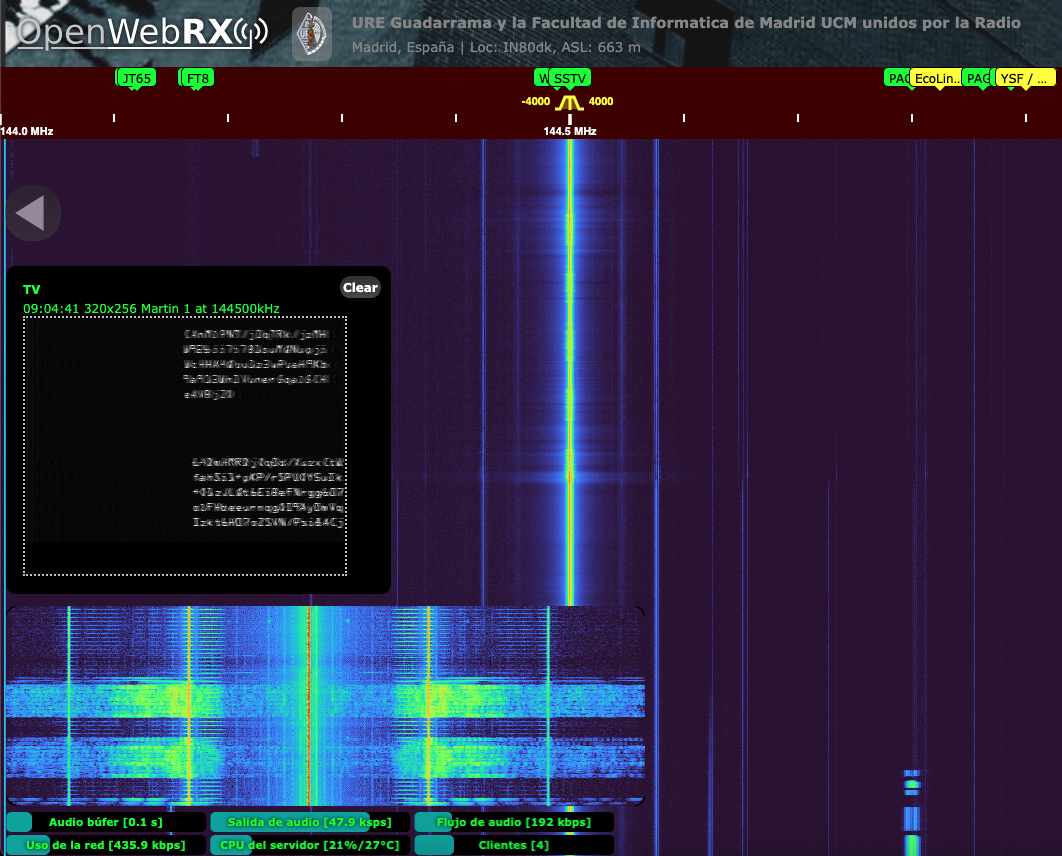
\includegraphics[width = 0.5 \textwidth]{Imagenes/pitea/nodo_radioescucha.png}
	\caption[Interfaz del nodo de radioescucha utilizado.]{Interfaz del nodo de radioescucha utilizado tras la decodificación de la señal SSTV mandada. Captura de pantalla.}
	\label{fig:nodo_radioescucha}
\end{figure}

\begin{figure}[h]
	\centering
	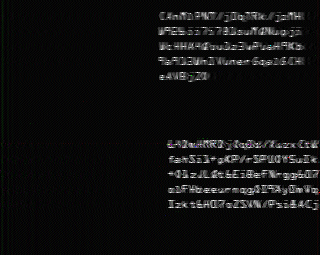
\includegraphics[width = 0.5 \textwidth]{Imagenes/pitea/nodo_radio.png}
	\caption[Imagen recuperada en la prueba de campo,~\ref{sec:transmision-rf}.]{Imagen recuperada en la prueba de campo,~\ref{sec:transmision-rf}. Generada por la herramienta.}
	\label{fig:nodo_radio}
\end{figure}

\section{Difusión en la red pública}
\label{sec:transmision-red_publica}
En esta sección se hablará de cómo se comportan los archivos portadores al ser transmitidos por la red pública.

\subsection{Generación de los archivos portadores}

Para esta sección se han generado varios archivos portadores con el fin de comprobar todas las funcionalidades de la herramienta. 
\begin{enumerate}
    \item \label{itm:audio-sin-cifrado} Audio portador sin cifrado, ocultador en imagen LSB y ocultador en audio LSB, figura~\ref{fig:gen_lsb}, generando~\ref{fig:collage_lsb_lsb}.
    \item \label{itm:audio-cifrado} Audio portador con cifrado AES, ocultador en imagen mediante el plasmado de texto en la imagen y ocultador en audio mediante su paso a audio codificado con SSTV, figura~\ref{fig:gen_radio}.

\end{enumerate}

\begin{figure}[h]
	\centering
	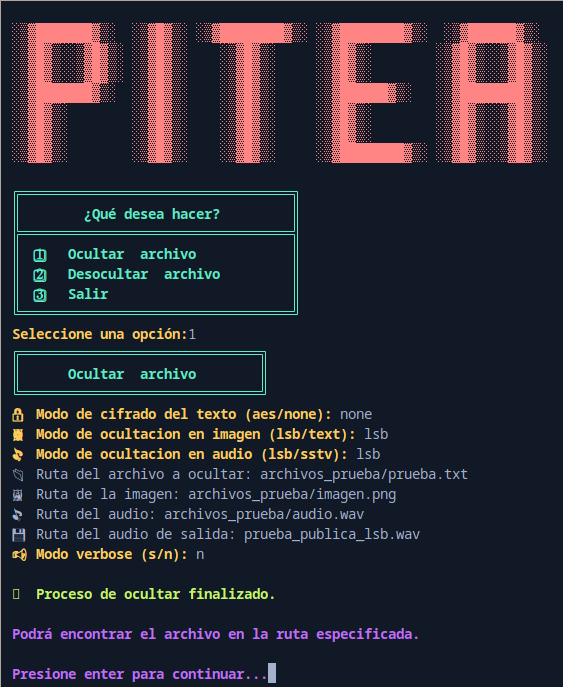
\includegraphics[width = 0.4 \textwidth]{Imagenes/pitea/gen_pub.png}
	\caption[Generación de audio portador, sin cifrado, LSB, LSB.]{Generación de audio portador, sin cifrado, LSB, LSB. Captura de pantalla de la herramienta.}
	\label{fig:gen_lsb}
\end{figure}

\begin{figure}[h]
	\centering
	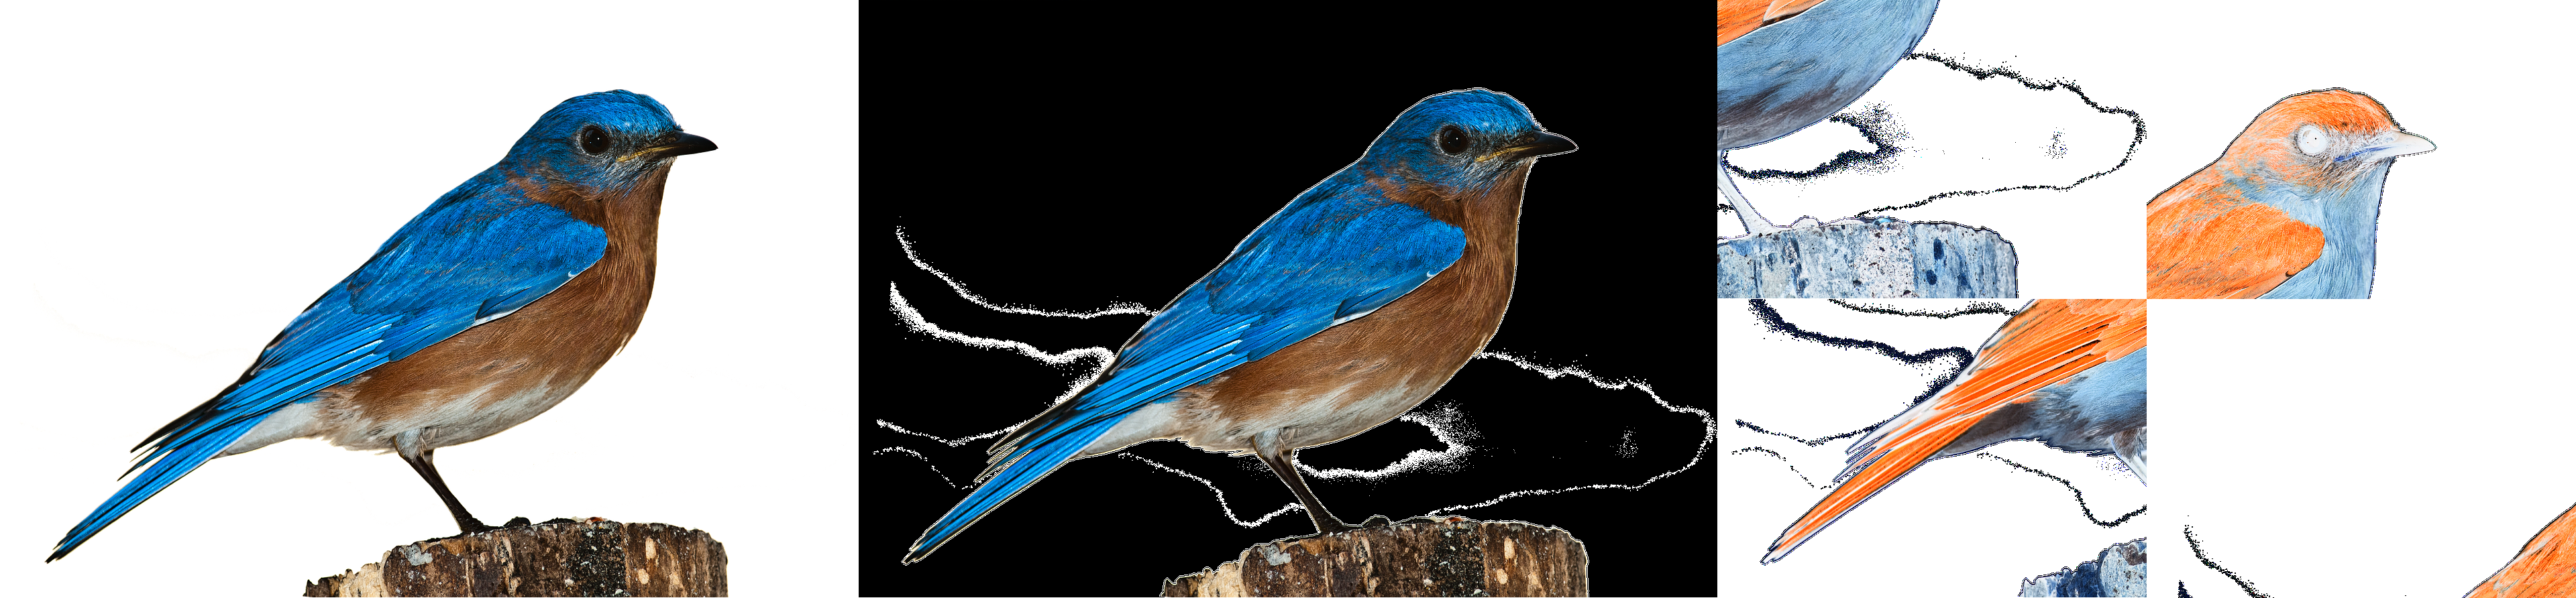
\includegraphics[width = 0.8\textwidth]{Imagenes/prueba_campo2_2/collage.png}
	\caption[\textit{Collage} de las imagenes sultante de la generación del archivo~\ref{itm:audio-sin-cifrado}.]{Imagenes resultantes de la generación del archivo~\ref{itm:audio-sin-cifrado}, imagen original, antes y después de la transformada respectivamente. Generadas por la herramienta.}
	\label{fig:collage_lsb_lsb}
\end{figure}
 
No se ha generado un archivo con ocultador en imagen LSB y ocultador en audio con SSTV debido a que SSTV es un formato sujeto a ruido, lo que significa que no es seguro que se recupere la imagen idéntica píxel a píxel, lo que hace que no se pueda recuperar el texto de la imagen de manera segura.\\


El audio~\ref{itm:audio-cifrado} se ha añadido a un vídeo para poder ser subido a TikTok.



\subsection{Resultado}

La primera prueba que se ha realizado es con el archivo~\ref{itm:audio-cifrado} en la cual se ha aprovechado la funcionalidad de captura de SSTV en \textit{streaming} para capturar el audio a la vez que se reproduce el video en TikTok, figura~\ref{fig:prueba1}. Tras la cual se ha generado la imagen ~\ref{fig:collage_streaming} donde se puede ver el antes y después de la transformada.\\

Los resultados son buenos, ya que el ojo humano puede reconocer los caracteres, haciendo que se pueda recuperar el texto original tras reconocer esos caracteres por el desocultador \textit{text} o transcribiendo la imagen a un archivo de texto y descifrándolo posteriormente, ambas soluciones implementadas en la herramienta.
\begin{figure}[h]
	\centering
	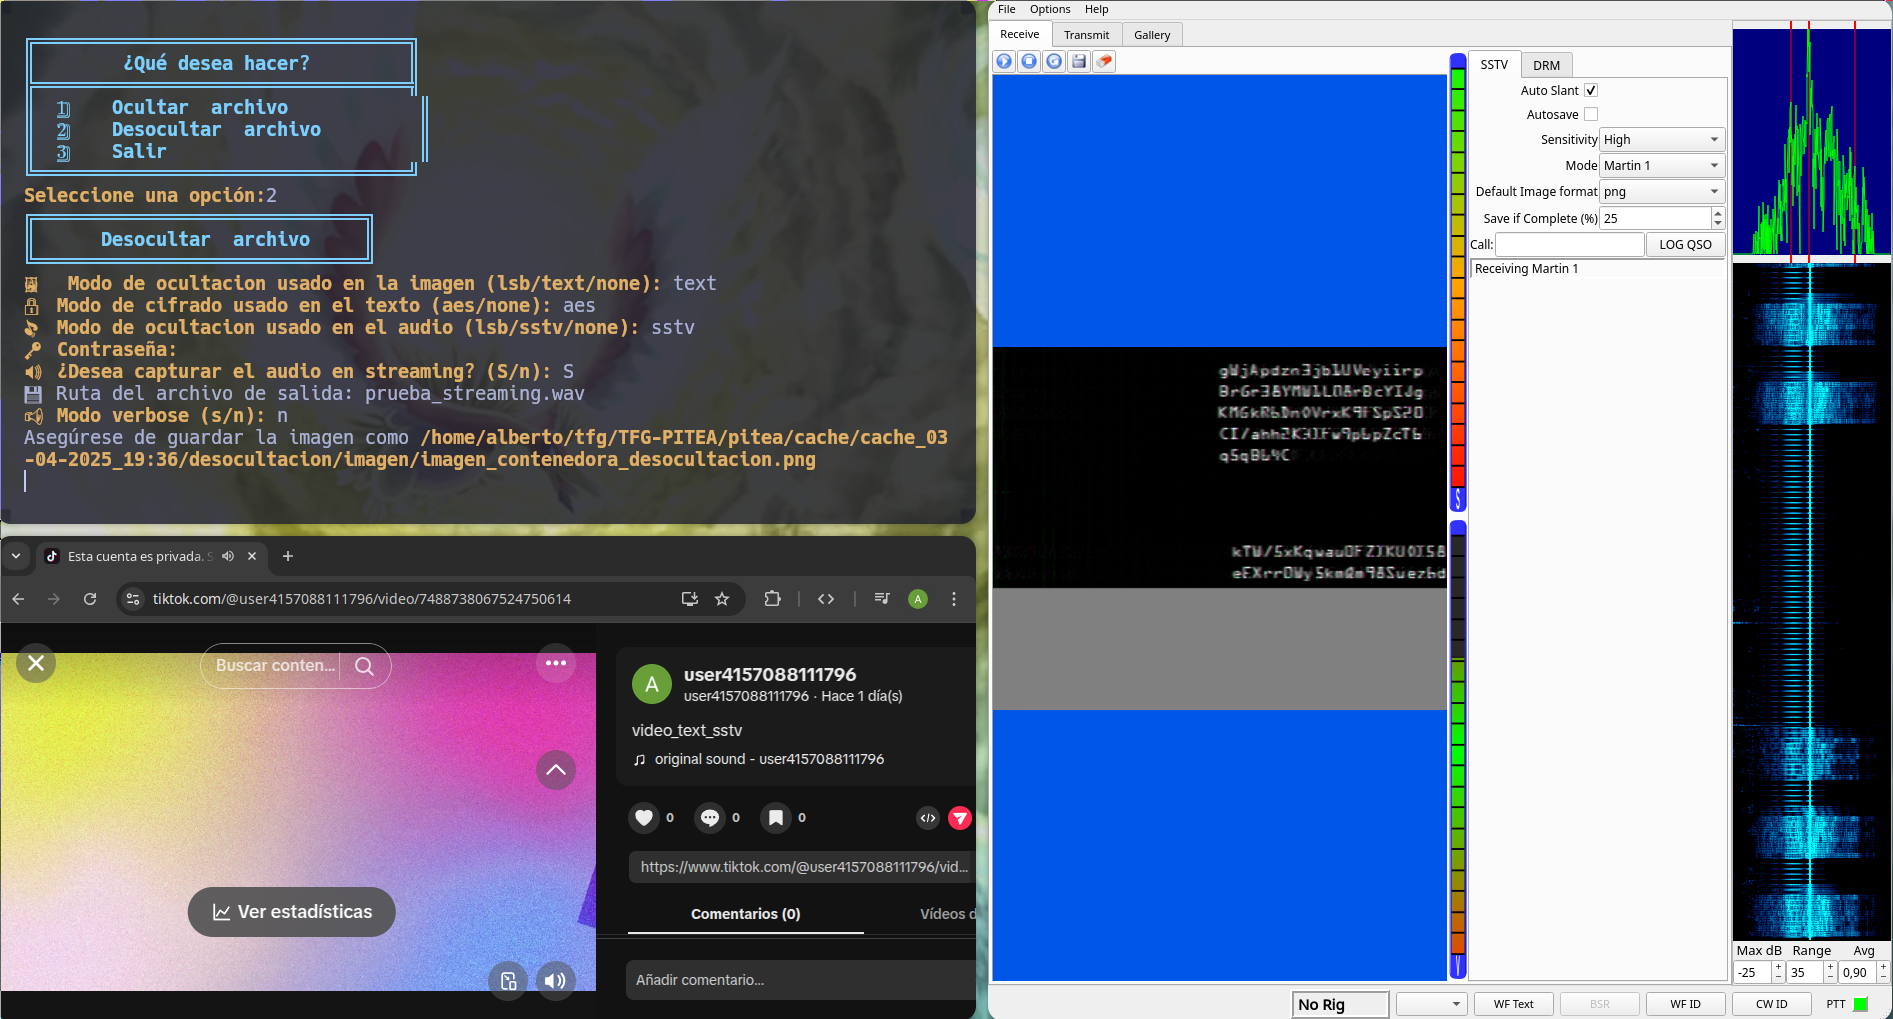
\includegraphics[width = 1\textwidth]{Imagenes/pitea/streaming.png}
	\caption[Captura en \textit{streaming} en Tiktok.]{Captura en \textit{streaming} en Tiktok, usando como decodificar QSSTV. \textit{Collage} formado por una captura de pantalla de la herramienta, arriba izquierda; interfaz de QSSTV, derecha; e interfaz web de TikTok, abajo izquierda.}
	\label{fig:prueba1}
\end{figure}

\begin{figure}[h]
	\centering
	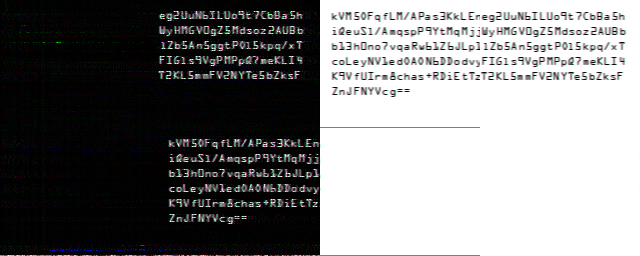
\includegraphics[width = 0.9\textwidth]{Imagenes/pitea/collage_streaming.png}
	\caption[Imagenes resultantes de la prueba con el archivo~\ref{itm:audio-cifrado}.]{Imagenes resultantes de la prueba con el archivo~\ref{itm:audio-cifrado}, antes y después de la transformada respectivamente. Generadas por la herramienta.}
	\label{fig:collage_streaming}
\end{figure}

La segunda prueba se ha realizado con el archivo~\ref{itm:audio-sin-cifrado}, ha consistido en ser mandado por WhatsApp, también podría haber sido cualquier servicio de correo que no comprima archivos multimedia, y al ser descargado ha sido pasado por la herramienta, dando como resultado las siguientes figuras:~\ref{fig:llamada_des} y~\ref{fig:collage2_lsb_lsb}.\\

El resultado es exitoso, ya que la salida de la herramienta, el archivo ``salida\_lsb\_lsb.txt'' como se puede ver en la figura~\ref{fig:llamada_des}, contiene: 
\begin{verbatim}
PITEA Protección de la informacíon mediante técnicas de esteganografía acústica
Alberto Martin Oruña y Rodrigo Gallego Marin
\end{verbatim}
que es exactamente igual al archivo inicial.

\begin{figure}[h]
	\centering
	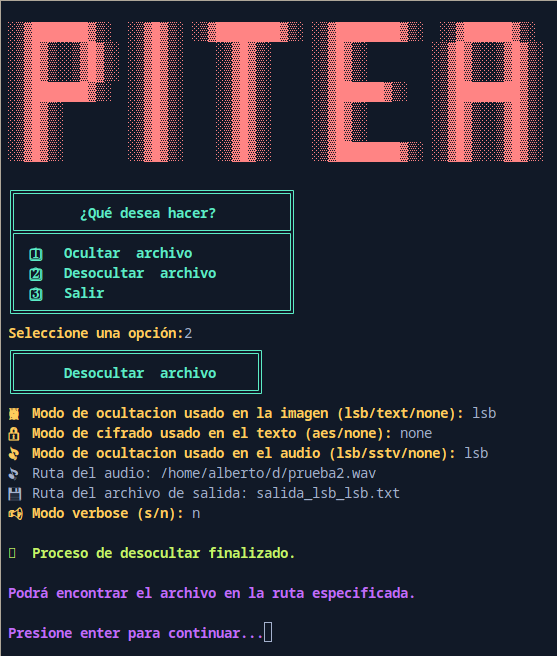
\includegraphics[width = 0.4\textwidth]{Imagenes/prueba_campo2_2/llamada.png}
	\caption[Llamada a la herramienta para la desocultación de ~\ref{itm:audio-sin-cifrado}.]{Llamada a la herramienta para la desocultación de ~\ref{itm:audio-sin-cifrado}. Captura de pantalla de la herramienta.}
	\label{fig:llamada_des}
\end{figure}

\begin{figure}[h]
	\centering
	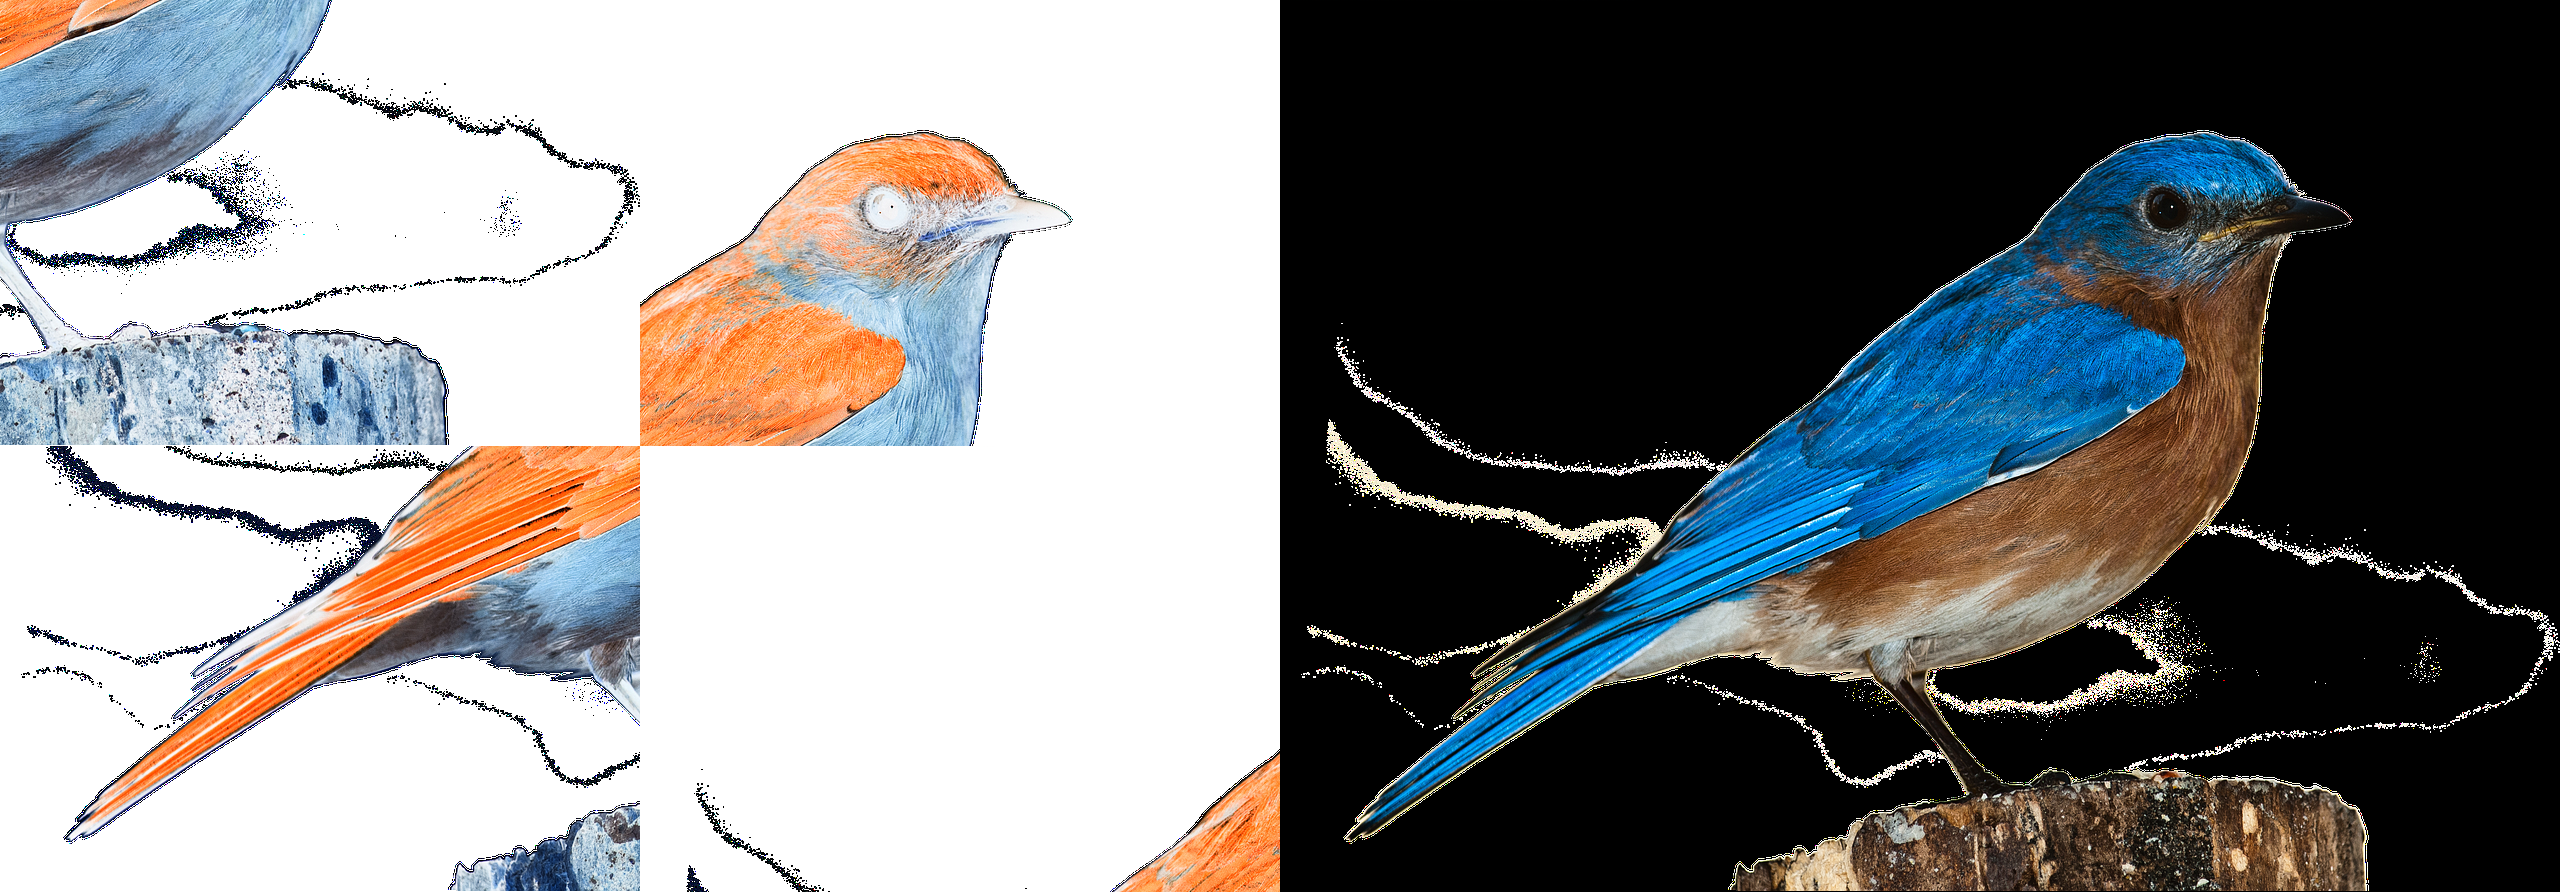
\includegraphics[width = 0.8\textwidth]{Imagenes/prueba_campo2_2/collage2.png}
	\caption[Imagenes resultantes de la desocultación del archivo~\ref{itm:audio-sin-cifrado}.]{Imagenes resultantes de la desocultación del archivo~\ref{itm:audio-sin-cifrado}, imagen recuperada en los LSB del audio e imagen destransformada respectivamente. Generadas por la herramienta.}
	\label{fig:collage2_lsb_lsb}
\end{figure}

\FloatBarrier
\newpage
\section{Análisis de \textit{OcultadorText}}
\label{sec:Analisis}
En esta sección se hablará de los análisis realizados sobre el ocultador en imágenes que se basa en el plasmado de texto en una imagen, tratando desde la generación de los conjuntos de datos utilizados hasta las conclusiones resultantes.\\

El análisis se ha dividido en dos partes, una por motor OCR usado, \textit{Tesseract-OCR} y \textit{EasyOCR}. Sin embargo, la estructura del experimento ha sido idéntica en ambos casos, solo variando los resultados. Las gráficas de cada parámetro han sido realizadas agrupando por ese parámetro y usando como función resumen la media aritmética. Se ha elegido la media frente a otras opciones como la mediana, valor máximo o valor mínimo, ya que el fin de este análisis es ver cuánto afecta cada variable al resultado, y el uso de la media como función resumen proporciona un valor representativo del comportamiento general..\\

En primer lugar se generó una lista de listas de palabras y números en inglés de tamaño aleatorio, entre 1 y 25, de longitud 10. Los números aparecen con un 5\% de probabilidad. Los componentes de esta lista serán los utilizados como los secretos que se van a ocultar.
Una vez generado el conjunto de secretos que vamos a procesar, se generó un conjunto de datos, \textit{dataset}, ejecutando el ocultador de imágenes correspondiente con tamaños de fuente entre 1 y 25 con un paso de 2, 10 fuentes tipográficas \footnote{Véase el apéndice \ref{Appendix:Fuentes} para ver las fuentes tipográficas concretas.} y una anchura máxima de imagen entre 800 píxeles y 10800 con paso 1000, estos intervalos y saltos han sido los interpretados como más relevantes y óptimos teniendo en cuenta las capacidades de cómputo que se tenían en el momento del experimento, ya que el uso de motores OCR consume muchos recursos hardware. Resultan dos \textit{datasets}\footnote{Se pueden encontrar en el repositorio de la herramienta \url{https://github.com/Alberto12x/PITEA/tree/main/experimental}.} similares a~\ref{tab:datsets}, siendo ``resultado'' la similitud entre el texto original y el texto extraído. La similitud ha sido calculada usando el algoritmo \textit{Gestalt Pattern Matching}.


\begin{table}[h]
	\centering
        \resizebox{\textwidth}{!}{
	\begin{tabular}{c|c|c|c|c|c}
		\textbf{Tamaño} & \textbf{Fuente} & \textbf{Anchura} & \textbf{Resultado} & \textbf{Texto original} & \textbf{Texto extraido} \\
		\hline\hline
		9 & OCR-a-std & 800 & 65.9 & hardpan... & harbpam... \\
		7 & OCRb & 1800 & 72.3 & quintary... & qunitary... \\
		5 & OCR-a-std & 4800 & 88.1 & depside... & deps1de... \\
		3 & OCRb & 3800 & 91.7 & unsaintlike... & unsa1nt1ike... \\
		1 & OCR-a-std & 2800 & 50.2 & cran drachm... & crarn drachm... \\
		7 & OCR-a-std & 6800 & 95.0 & isothiocyano... & isothiocvano... \\
		3 & OCR-a-std & 9800 & 92.4 & unmapped... & unmapp3d... \\
		5 & Arial & 8800 & 87.5 & diluvianism... & diluv1an1sm... \\
		9 & OCR-a-std & 7800 & 93.2 & hardpan diluvianism... & harclpan diluian1sm... \\
		1 & OCR-a-std & 800 & 41.8 & drachm... & draclm... \\
		\hline
	\end{tabular}
    }
	\caption[Ejemplo de \textit{datasets} generados]{Ejemplo de \textit{datasets} generados.}
	\label{tab:datsets}
\end{table}
\newpage

\subsection{Análisis de \textit{Tesseract-OCR}}
\label{sec:t}

Lo primero a mencionar en este análisis es que la herramienta no detecta espacios en blanco, por lo que se ha calculado la similitud entre los textos originales y los extraídos eliminándolos.\\

El primer análisis que se ha realizado es ver cómo afecta el tamaño de la fuente al resultado, figura~\ref{fig:t_tam}. En la gráfica se puede apreciar cómo con tamaños de fuentes inferiores a 7, los textos extraídos no tienen ninguna similitud con los originales o simplemente no se ha extraído ningún texto. Entre un tamaño de 7 a 9 la herramienta empieza a detectar mejor los textos y es a partir de un tamaño de fuente 11 cuando la herramienta alcanza resultados óptimos superando el 95\% de similitud y a partir de 17 se alcanza una similitud casi del 100\%.\\

\begin{figure}[h]
	\centering
	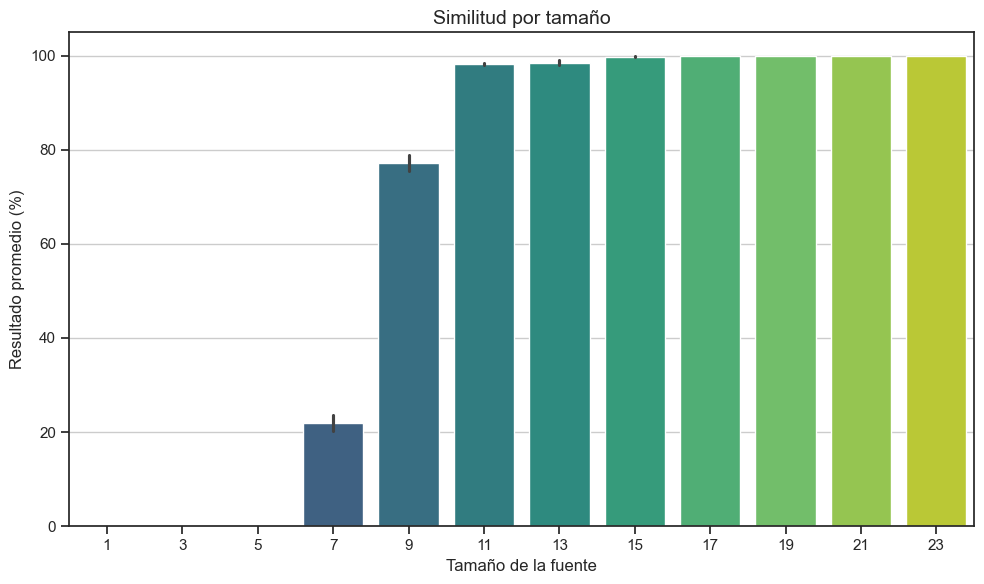
\includegraphics[width = 0.7\textwidth]{Imagenes/experimentos/t_tam.png}
	\caption[Gráfica de resultado por tamaño de la fuente utilizada. \textit{Tesseratc-OCR}.]{Gráfica de resultado (\%) variando el tamaño de la fuente utilizada, agrupando por ello y calculando la media del resultado para cada grupo. \textit{Tesseratc-OCR}. Elaboración propia.}
	\label{fig:t_tam}
\end{figure} 
El siguiente análisis que se realizó fue ver cómo las tipografías utilizadas afectaban a la herramienta, figura~\ref{fig:t_fuen}. En la gráfica se puede ver que aunque se ven pequeñas variaciones en los resultados, estas no son superiores al 15\% por lo que la fuente tipográfica utilizada no afecta de manera significativa al resultado. Es de resaltar que las fuentes específicas para motores OCR no destacan sobre el resto, siendo posible que esto se deba a las fuentes elegidas para entrenar \textit{tesseract-OCR}.\\ 





Posteriormente se analizó el efecto que tenía la anchura máxima de las imágenes generadas en el resultado, esto debido a que dependiendo de la anchura, la cantidad de palabras por línea varía. En su gráfica, figura \ref{fig:t_anch}, se puede ver que no afecta de manera significativa en el resultado, ya que tanto sus valores medios como márgenes de error son idénticos o muy parecidos, siendo solo necesario que la anchura máxima sea igual o mayor que el carácter más ancho del mensaje.\\

Se siguió graficando todos los parámetros a la vez, figura~\ref{fig:t_scatt}. En esta gráfica, de 5 dimensiones, se ha utilizado el color, la forma el tamaño de los puntos como dimensiones extra. Se puede apreciar que el único parámetro relevante es el tamaño de la fuente, ya que solo se aprecian cambios al recorrer ese eje.\\


\begin{figure}[h]
	\centering
	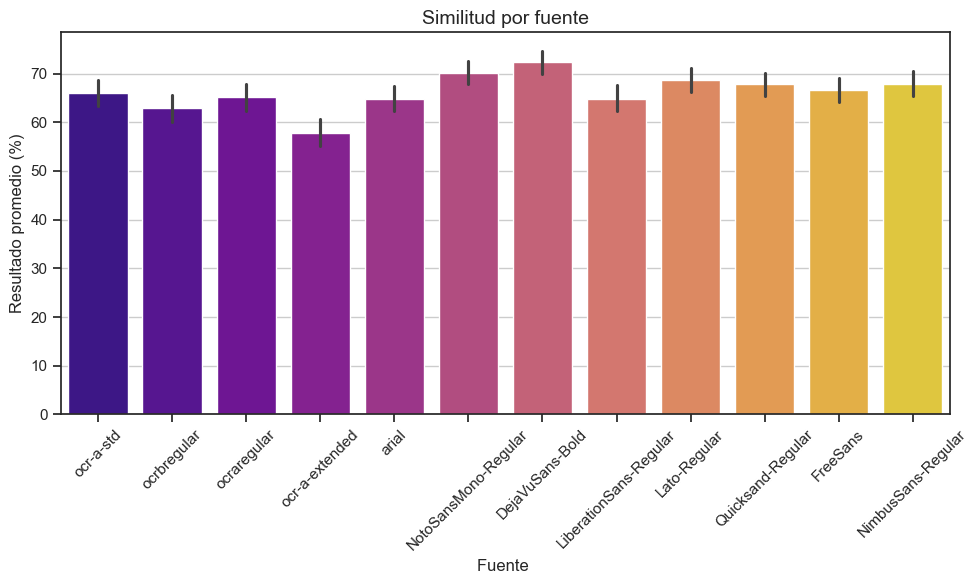
\includegraphics[width = 0.7\textwidth]{Imagenes/experimentos/t_fuen.png}
	\caption[Gráfica de resultado por fuente utilizada. \textit{Tesseratc-OCR}.]{Gráfica de resultado (\%) variando la fuente utilizada, agrupando por ella y calculando la media del resultado para cada grupo. \textit{Tesseratc-OCR}.  Elaboración propia.}
	\label{fig:t_fuen}
\end{figure}

\begin{figure}[h]
	\centering
	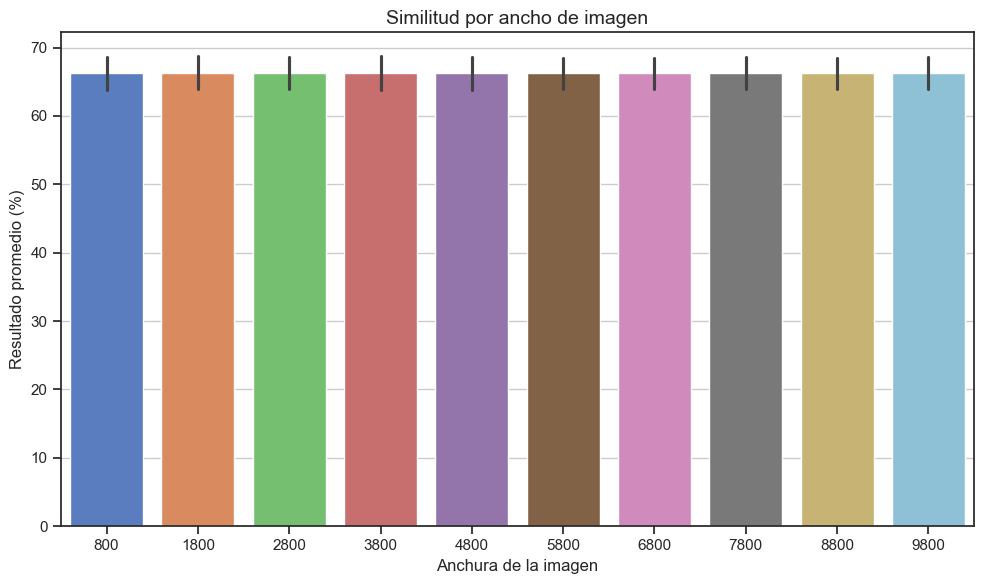
\includegraphics[width = 0.7\textwidth]{Imagenes/experimentos/t_anch.png}
	\caption[Gráfica de resultado por anchura de la imagen. \textit{Tesseratc-OCR}. ]{Gráfica de resultado (\%) variando la anchura de la imagen utilizada, agrupando por ella y calculando la media del resultado para cada grupo. \textit{Tesseratc-OCR}.  Elaboración propia.}
	\label{fig:t_anch}
\end{figure}

Para finalizar los análisis sobre este motor, se analizó si la longitud del mensaje a ocultar y la existencia de números afectaban al resultado, figura~\ref{fig:t_num}. Se puede concluir que ninguna de las dos variables mencionadas afecta al resultado, ya que no se aprecian cambios al recorrer sus ejes.\\



Tras este análisis se puede concluir que el tamaño de la fuente tipográfica utilizado es lo que más afecta a la precisión de la herramienta, afectando el resto de parámetros de manera casi superflua, pero siendo necesarios ya que la desocultación se puede realizar también sin motor OCR, usando el ojo humano.

\begin{figure}[h]
	\centering
	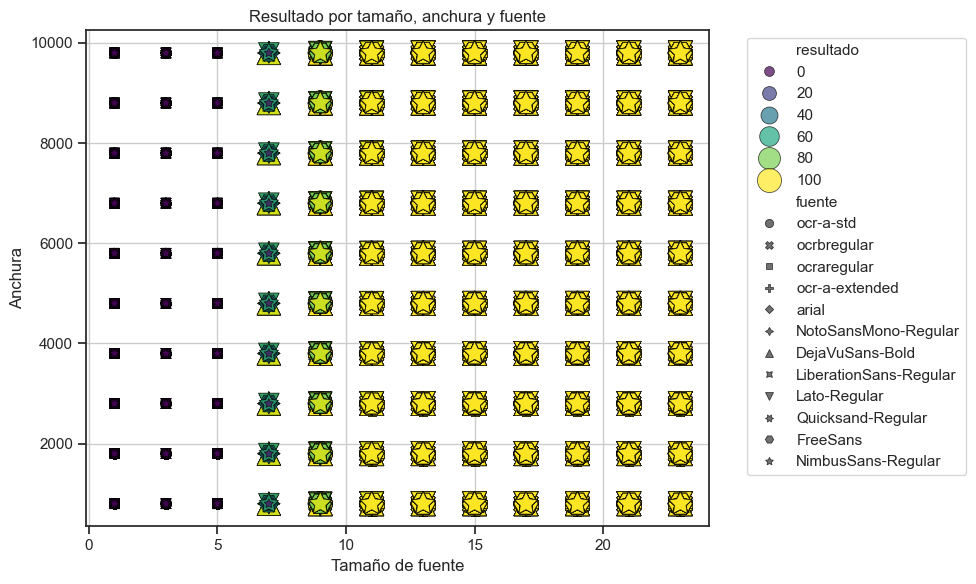
\includegraphics[width = 0.7\textwidth]{Imagenes/experimentos/t_scatt.png}
	\caption[Gráfica de todos los parámetros configurables. \textit{Tesseratc-OCR}.]{Gráfica de todos los parámetros configurables. \textit{Tesseratc-OCR}.  Elaboración propia.}
	\label{fig:t_scatt}
\end{figure}




\begin{figure}[h]
	\centering
	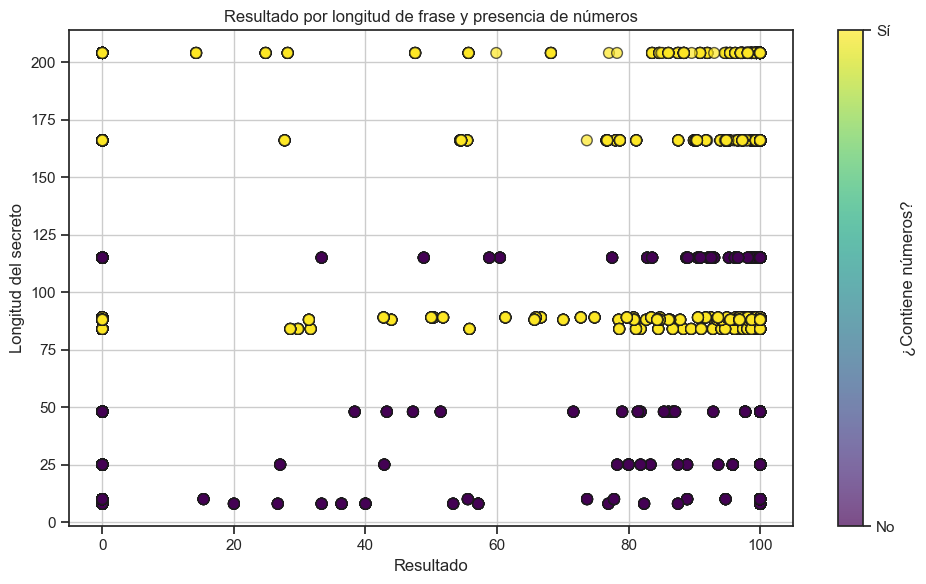
\includegraphics[width = 0.7\textwidth]{Imagenes/experimentos/t_num.png}
	\caption[Gráfica de resultado por longitud y números. \textit{Tesseratc-OCR}.]{Gráfica de resultado (\%) variando la longitud del secreto y el contenido numérico. \textit{Tesseratc-OCR}.  Elaboración propia.}
	\label{fig:t_num}
\end{figure}


\FloatBarrier
\subsection{Análisis de \textit{EasyOCR}}

Manteniéndose la misma estructura del análisis de la sección~\ref{sec:t}, se empezó estudiando la influencia del tamaño de la fuente tipográfica en el resultado, figura~\ref{fig:e_tam}. En esa gráfica se puede ver una tendencia bastante lineal a resultados mayores según se aumenta el tamaño de la fuente, además de que los mejores resultados obtenidos rondan el 60\%.\\



Continuando, en la figura~\ref{fig:e_fuen} se puede ver que la fuente utilizada no varía demasiado el resultado, un 10\% en el mayor de los casos. Es cuanto menos curioso que las fuentes específicas para OCR tampoco destacan en este motor.\\



En la figura~\ref{fig:e_anch} se puede ver cómo el ancho de la figura afecta negativamente al resultado, siendo las imágenes más anchas las que peor resultado 
ofrecen.\\

\begin{figure}[h]
	\centering
	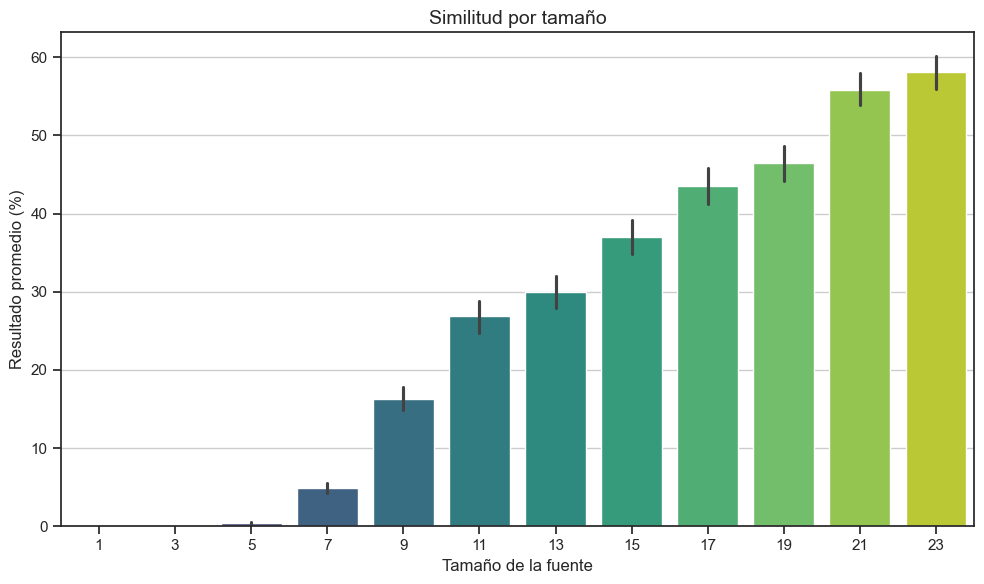
\includegraphics[width = 0.7\textwidth]{Imagenes/experimentos/e_tam.png}
	\caption[Gráfica de resultado por tamaño de la fuente utilizada. \textit{EasyOCR}.]{Gráfica de resultado (\%) variando el tamaño de la fuente utilizada, agrupando por ello y calculando la media del resultado para cada grupo. \textit{EasyOCR}. Elaboración propia.}
	\label{fig:e_tam}
\end{figure}

\begin{figure}[h]
	\centering
	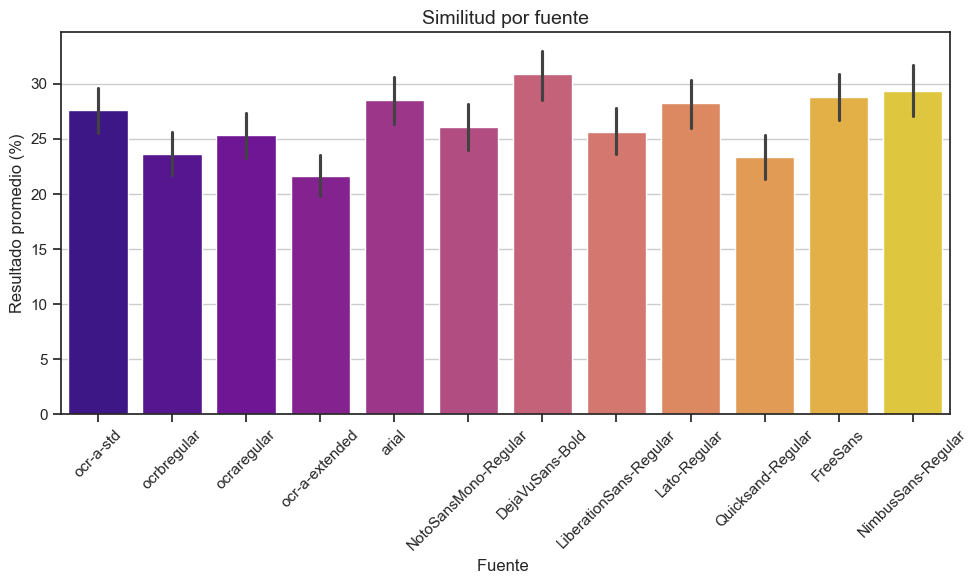
\includegraphics[width = 0.7\textwidth]{Imagenes/experimentos/e_fuen.png}
	\caption[Gráfica de resultado por fuente utilizada. \textit{EasyOCR}.]{Gráfica de resultado (\%) variando la fuente utilizada, agrupando por ella y calculando la media del resultado para cada grupo. \textit{EasyOCR}. Elaboración propia.}
	\label{fig:e_fuen}
\end{figure}


En el caso de la figura~\ref{fig:e_scatt}, se volvieron a visualizar todos los parámetros utilizando formas, colores y tamaños como dimensiones extras. Se puede ver lo anteriormente mencionado que los resultados, color y tamaño, mejoran según aumenta el tamaño de la fuente y disminuye la anchura de la imagen. Además, se puede apreciar que en valores intermedios de tamaños y anchuras, ciertas fuentes son mejores que otras, como el caso de \textit{FreeSans} con tamaño 10 y anchura 6000 píxeles.\\



Dada la tendencia a mejorar resultados aumentando el tamaño de la fuente, se decidió aumentar el \textit{dataset} para ver cómo evoluciona esa tendencia, pero esta vez solo usando una fuente y una anchura de imagen óptima para reducir la carga de trabajo al equipo encargado de generarlo. El resultado es la figura~\ref{fig:e_tam_extra} donde se puede ver que la tendencia a mejorar resultados se vuelve monótona a partir de un tamaño superior a 20 aproximadamente, experimentando cambios mínimos a partir de ese punto. Además, de manera indirecta se puede ver que el resultado asciende hasta el 80\% usando las configuraciones adecuadas.

\begin{figure}[h]
	\centering
	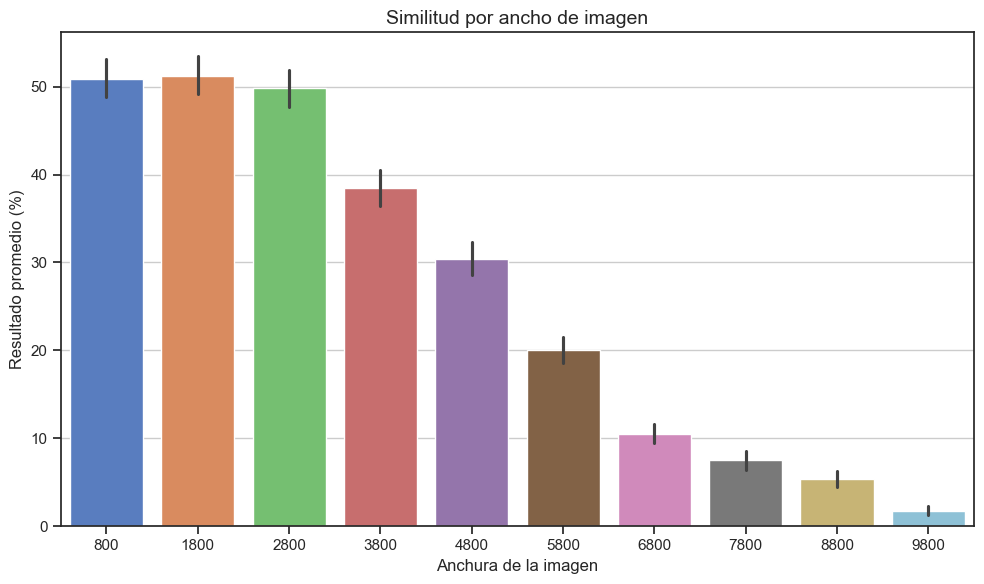
\includegraphics[width = 0.7\textwidth]{Imagenes/experimentos/e_anch.png}
	\caption[Gráfica de resultado por anchura de la imagen utilizada. \textit{EasyOCR}.]{Gráfica de resultado (\%) variando la anchura de la imagen utilizada, agrupando por ella y calculando la media del resultado para cada grupo. \textit{EasyOCR}.  Elaboración propia.}
	\label{fig:e_anch}
\end{figure}



\begin{figure}[h]
	\centering
	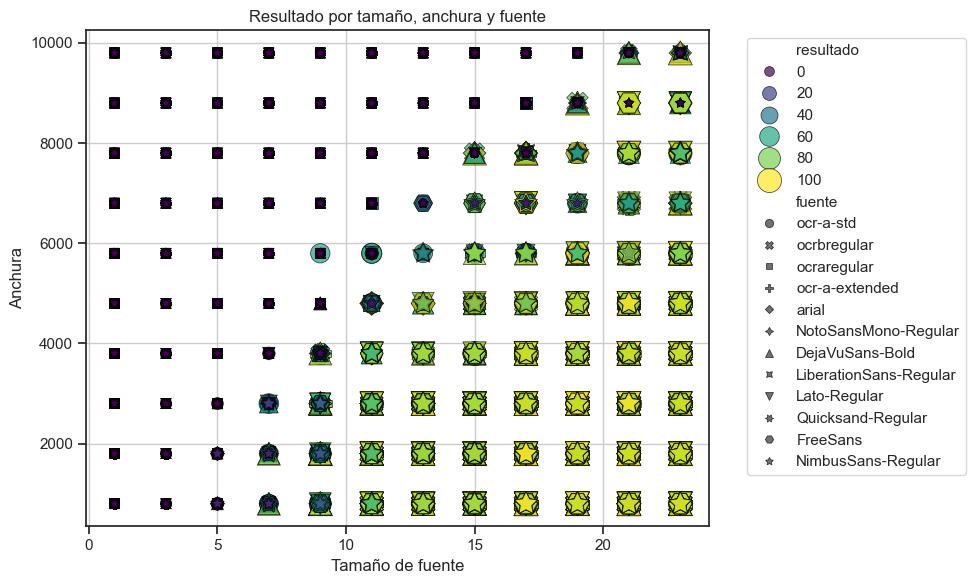
\includegraphics[width = 0.7\textwidth]{Imagenes/experimentos/e_scatt.png}
	\caption[Gráfica de todos los parámetros configurables. \textit{EasyOCR}.]{Gráfica de todos los parámetros configurables. \textit{EasyOCR}.  Elaboración propia.}
	\label{fig:e_scatt}
\end{figure}

Tras el análisis, podemos concluir que los parámetros introducidos varían de manera significativa el resultado, por lo que es importante tenerlos en cuenta al ejecutar la herramienta.

\begin{figure}[h]
	\centering
	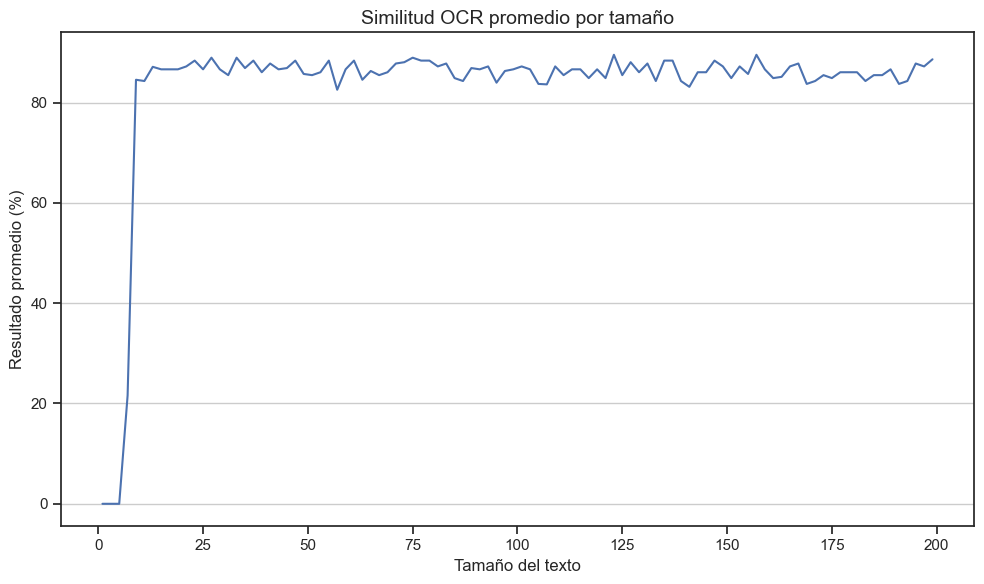
\includegraphics[width = 1\textwidth]{Imagenes/experimentos/e_tam_extra.png}
	\caption[Gráfica de todos los parámetros configurables. \textit{EasyOCR}.]{Gráfica de resultado (\%) variando el tamaño de la fuente utilizada y usando el resto de parámetros con sus valores más eficaces. Fuente tipográfica: DejaVuSans-Bold y anchura de imagen 800 píxeles. \textit{EasyOCR}. Elaboración propia.}
	\label{fig:e_tam_extra}
\end{figure}


